\chapter{REALM Demonstration}
% Main Gist 
% - Demonstrate OpenMC problem with REALM. 
% Structure 
% - realm demonstration of OpenMC Coupling for a toy problem. 
In this chapter, I demonstrate \gls{REALM}'s capabilities with a simple neutronics 
problem. 

\section{Straightened AHTR Fuel Slab}
\subsection{Problem Definition}
I explore how inhomogeneous fuel distributions impact $k_{eff}$ compared to 
homogenous fuel distributions that are customary in most reactor designs. 
The reactor core explored is a straightened slab from the \gls{FHR} benchmark's
\gls{AHTR} design.
Figure \ref{fig:straightened_slab} illustrates the straightened fuel slab. 
\begin{figure}[]
    \centering
    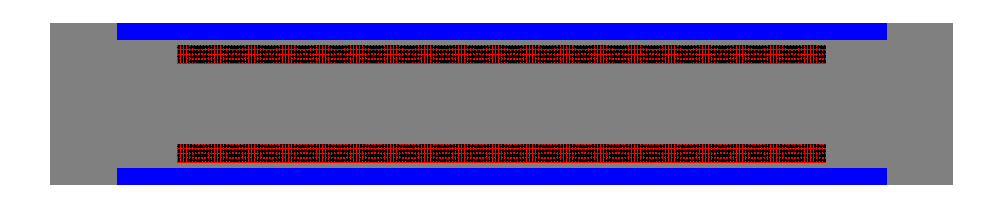
\includegraphics[width=\linewidth]{straightened_slab.png}
    \raggedright
    \resizebox{0.3\textwidth}{!}{
        \hspace{1cm}
        \fbox{\begin{tabular}{ll}
            \textcolor{fhrblue}{$\blacksquare$} & FliBe \\
            \textcolor{fhrgrey}{$\blacksquare$} & Graphite (Fuel Plank)\\
            \textcolor{fhrred}{$\blacksquare$} & Graphite (Fuel Stripe) \\
            \textcolor{fhrblack}{$\blacksquare$} & TRISO particle 

            \end{tabular}}}
    \caption{Straightened \acrfull{AHTR} fuel slab.}
    \label{fig:straightened_slab}
\end{figure}
The slab has dimensions of $27.1 \times 3.25 \times 1.85\ cm^3$
with periodic boundary conditions in the x and y directions and reflective 
boundary conditions in the z direction. 
The materials are the same as in the \gls{FHR} benchmark, with the exception 
of the homogenization of each \gls{TRISO} particle's four outer layers: 
porous carbon buffer, inner pyrolytic carbon, silicon carbide layer, and the 
outer pyrolitic carbon. 
The \gls{TRISO} particles' dimensions remain the same.
The $k_{eff}$ for this original straighted \gls{AHTR} configuration is 
$1.38625 +/- 0.00109$. 

The \gls{REALM} optimization problem's objective is to maximize the slab's 
$k_{eff}$, by varying the \gls{TRISO} particle packing fraction across the slab,
while keeping total \gls{TRISO} particle total packing fraction constant at 0.0979. 
This total packing fraction is consistent with the original straightened slab with 
TRISO particles in fuel stripes (Figure \ref{fig:straightened_slab}). 
The slab is divided into ten slices along the x axis between the FliBe and graphite 
buffers resulting in ten $2.31 \times 2.55 \times 1.85\ cm^3$ slices. 
The \gls{TRISO} particle packing fraction's distribution across slices is 
governed by a sine distribution: 
\begin{align}
    PF(x) &= (a\ sin(bx + c) + 2) \times NF\\
    \intertext{where}
    a, b, c &= \mbox{constants that control sine function's shape} \nonumber \\
    x &= \mbox{midpoint value for each slice} \nonumber \\
    NF &= \mbox{Normalization factor} \nonumber
\end{align}
The sine distribution's value at each of the ten x-slices' midpoints are collected and 
normalized by the total packing fraction to ensure that there is a consistent 
amount of \gls{TRISO} particles in the slab. 
Thus, for a packing fraction distribution of 
$PF(x) = (0.5\ sin(\frac{\pi}{3}x + \pi) + 2)  \times NF$. 
The packing fraction for the ten slices are 0.103, 0.120, 0.049, 0.138, 
0.076, 0.081, 0.136, 0.048, 0.125, 0.098, respectively. 
Figure \ref{fig:triso_distribution} shows a plot of this sine distribution, highlights 
the packing fraction at the respective midpoints, and an xy view of the slab
with packing fraction varying based on this sine distribution. 
\begin{figure}[]
    \centering
    \makebox[\textwidth][c]{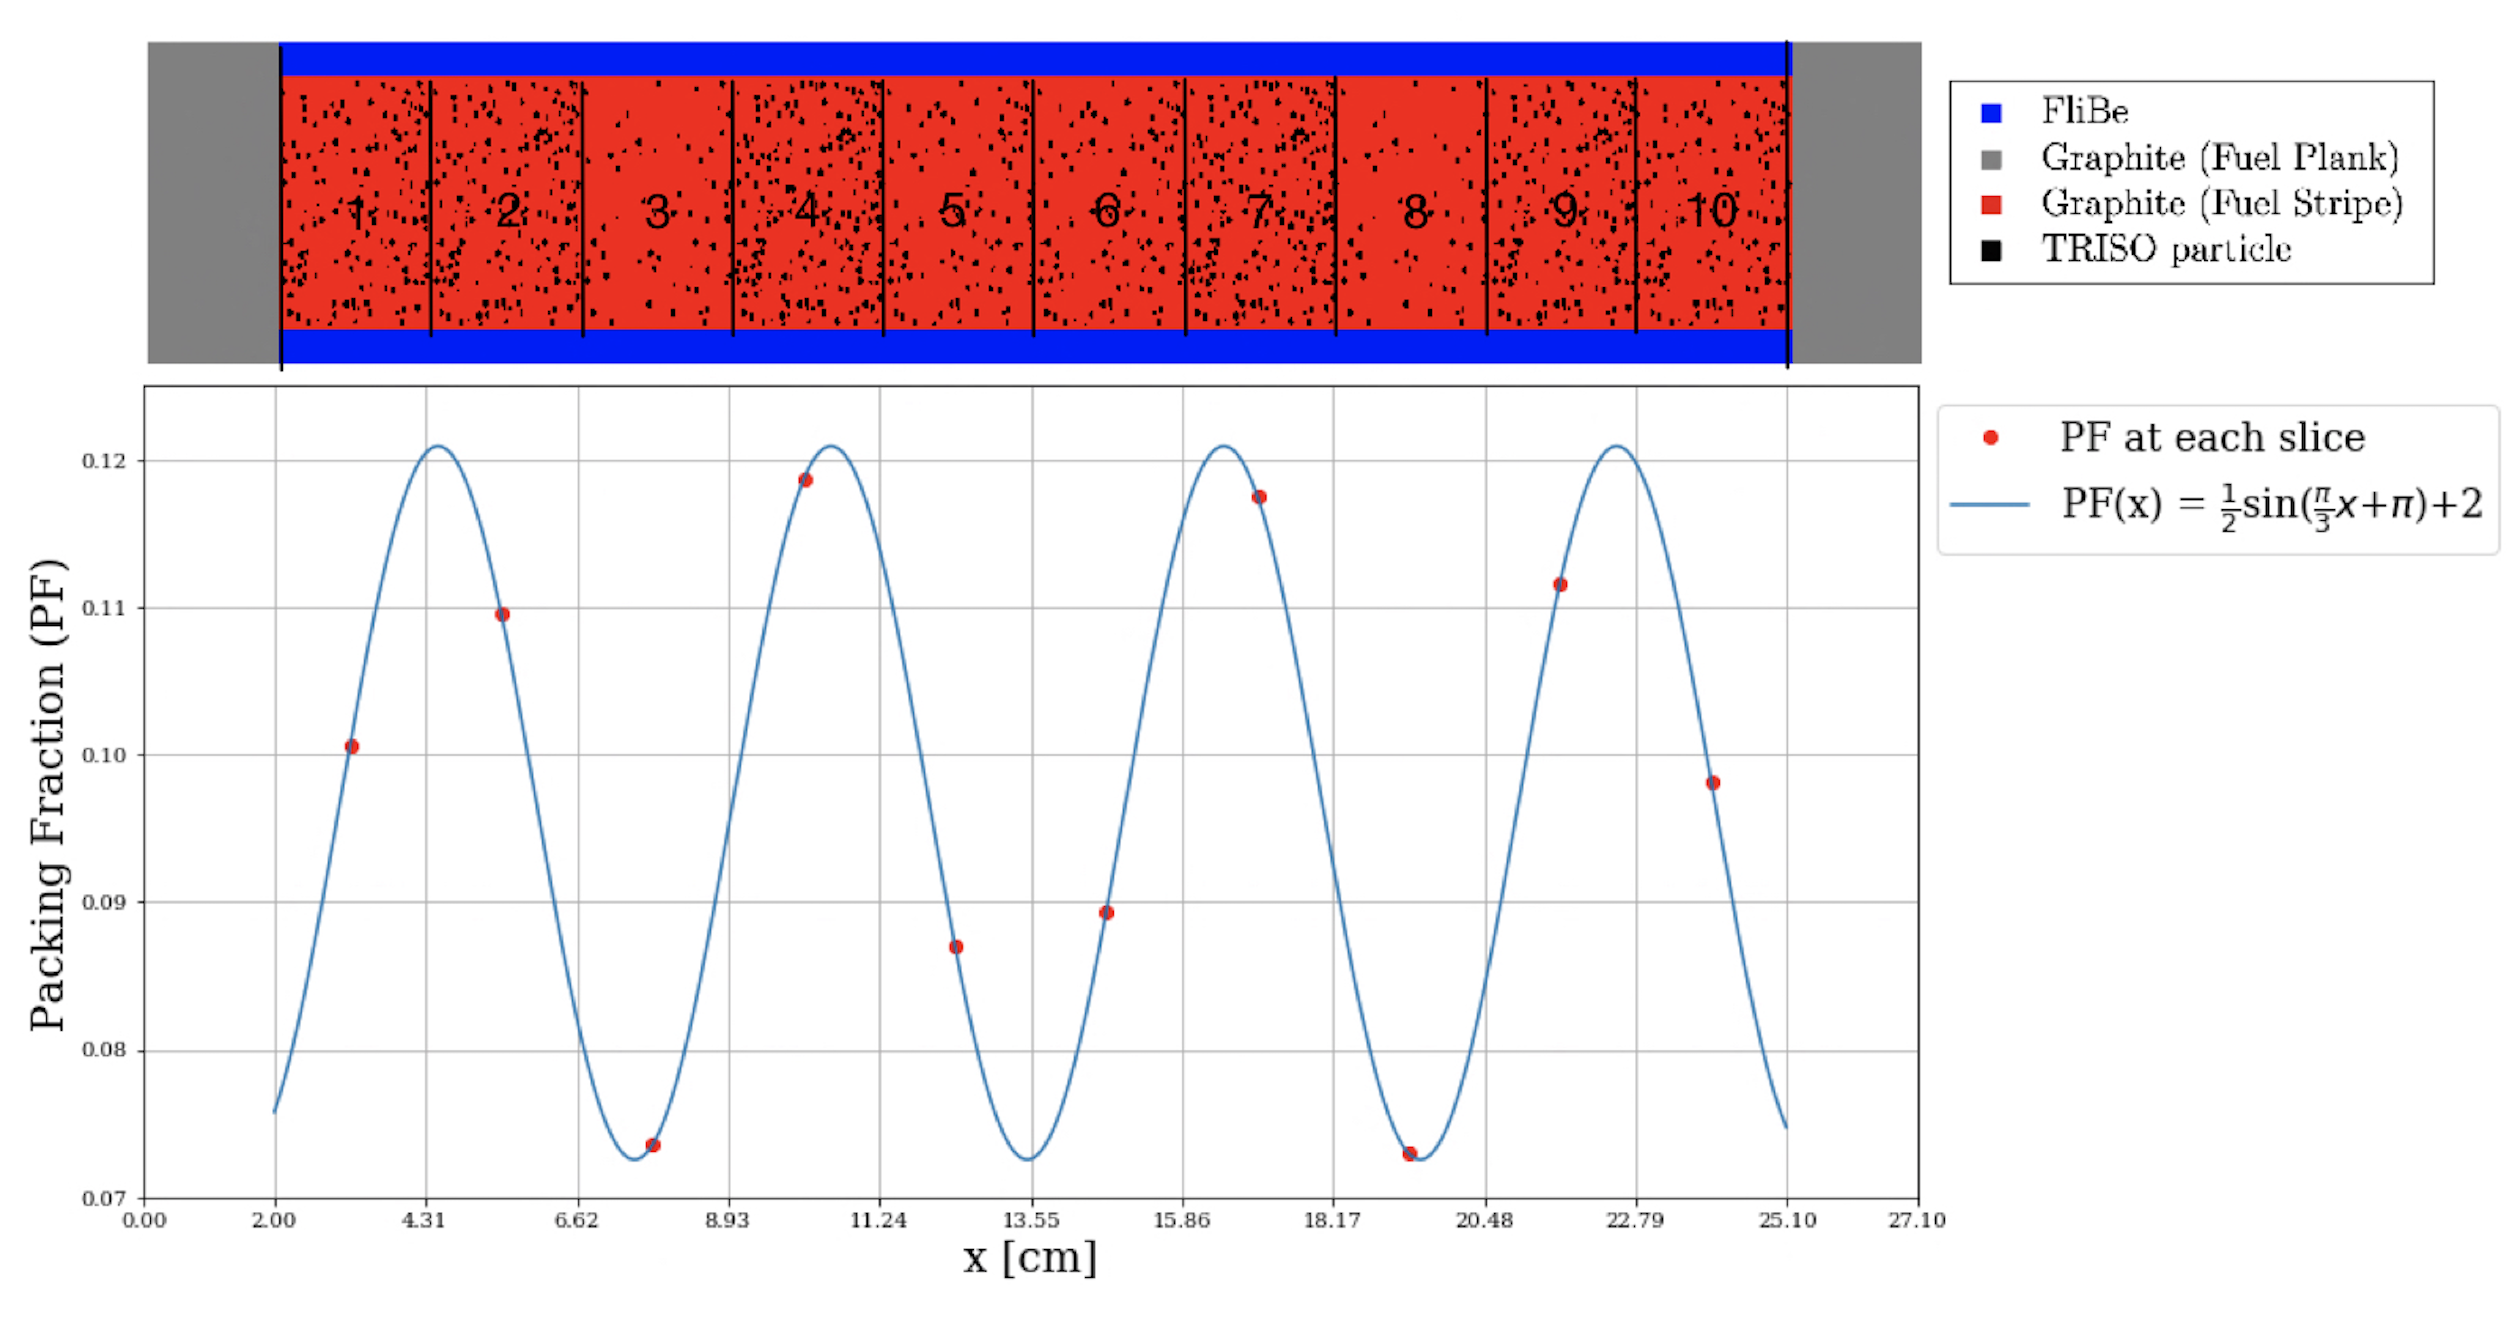
\includegraphics[width=1.1\linewidth]{triso_distribution_sine.png}} 
    \caption{Below: $PF(x) = (0.5\ sin(\frac{\pi}{3}x + \pi) + 2)  \times NF$ 
    sine distribution with red points indicating the packing fraction at each slice. 
    Above: Straightened \acrlong{AHTR} fuel slab with varying \gls{TRISO} particle 
    distribution across ten slices based on the sine distribution. }
    \label{fig:triso_distribution}
\end{figure}
The genetic algorithm varies the $a$, $b$ and $c$ variables to find a combination 
that maximizes the average $k_{eff}$ of the genetic algorithm's final generation 
of $a$, $b$ and $c$ combinations.
The OpenMC evaluator calculates $k_{eff}$. 
Each OpenMC simulation is run with 80 active cycles, 20 inactive cycles, and 
8000 particles to reach an uncertainty of approximately 130pcm. 

\subsection{Hyperparameter Search}
I conducted a hyperparameter search with random sampling. 
I used random search over grid search because of the former's efficiency in 
high-dimensional spaces. 
Figure \ref{fig:random_vs_grid_sampling} illustrates how grid sampling gives 
even coverage in the original 2-d space, but provides inefficient coverage in 
projections onto either the x1 or x2 subspace.  
In contrast, random sampling has slightly less evenly distributed in the original 
space, but far more evenly distributed in the subspaces.
\begin{figure}[]
    \centering
    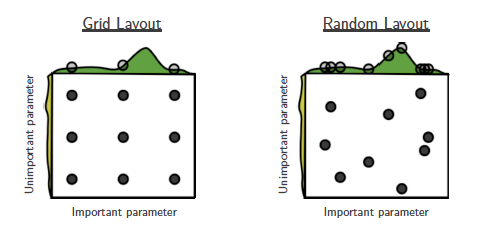
\includegraphics[width=0.8\linewidth]{random_vs_grid_sampling.png} 
    \caption{The impact of grid sampling vs random sampling on coverage of projections 
    into subspaces (reproduced from \cite{}). Random sampling has better coverage 
    in the subspaces.}
    \label{fig:random_vs_grid_sampling}
\end{figure}
The hyperparameters varied include: population size, number of generations, 
mutation probability, mating probability, selection operator, selection operator's 
k value, selection operator's tournament size, mutation operator, and mating 
operator.  

I used random sampling with a coarse-to-fine sampling scheme, previously 
discussed in Chapter \ref{chap:lit-review} to perform the hyperparameter search. 
I started with 25 coarse experiments and fine tuned the hyperparameters
with 15 fine experiments. 
% explain more about 1000 evaluations gen and pop size. 
Table \ref{tab:hyperparameter_search} shows the lower and upper bounds used 
for random sampling of each hyperparameter. 
\begin{table}[]
    \centering
    \onehalfspacing
    \caption{Hyperparameters}
	\label{tab:hyperparameter_search}
    \footnotesize
    \begin{tabular}{p{4cm}lp{3.4cm}p{3.4cm}p{3.4cm}}
    \hline 
    \textbf{Hyperparameter}& \textbf{Type} & \textbf{Coarse Search Bounds} & \textbf{Fine Search 1 Bounds} & \textbf{Fine Search 2 Bounds} \\
    \hline
    Experiments & - & 0 to 24 & 24 to 34 & 35 to 39 \\ 
    \hline
    Population size (pop) & Continuous & 10 $<$ x $<$ 100 & 20 $<$ x $<$ 60 & 60 \\ 
    Mutation probability & Continuous & 0.1 $<$ x $<$ 0.4 & 0.2 $<$ x $<$ 0.4& 0.2 $<$ x $<$ 0.3\\
    Mating probability & Continuous & 0.1 $<$ x $<$ 0.6 &  0.1 $<$ x $<$ 0.3 &  0.45 $<$ x $<$ 0.6\\
    Selection operator & Discrete & \texttt{SelTournament}, \texttt{SelBest}, \texttt{SelNSGA2} & \texttt{SelTournament}, \texttt{SelBest}, \texttt{SelNSGA2}& \texttt{SelTournament}\\
    Selection individuals & Continuous & $\frac{1}{3}pop$ $<$ x $<$ $\frac{2}{3}pop$ & $\frac{1}{3}pop$ $<$ x $<$ $\frac{2}{3}pop$ & 15\\
    Selection tournament size (only for SelTournament) & Continuous & 2 $<$ x $<$ 8 &2 $<$ x $<$ 8&5\\
    Mutation Operator & Discrete & \texttt{mutPolynomialBounded} &\texttt{mutPolynomialBounded}&\texttt{mutPolynomialBounded}\\
    Mating Operator & Discrete& \texttt{cxOnePoint}, \texttt{cxUniform}, \texttt{cxBlend} &\texttt{cxOnePoint}, \texttt{cxUniform}, \texttt{cxBlend}&\texttt{cxOnePoint}, \texttt{cxBlend}\\ 
    \hline
    \end{tabular}
\end{table}

The objective of the initial 25 coarse experiments is to narrow down the 
hyperparameters to find optimal hyperparameter bounds that produce a
higher average $k_{eff}$ values in each experiment's final generation. 
Figure \ref{fig:hyperparameter_sens} shows the hyperparameters' plotted against 
each other with a third color dimension of the average $k_{eff}$ value in each 
experiment's final generation. 
The lighter the scatter point is, the larger the final population's 
average $k_{eff}$ value is, thus the better the hyperparameter set. 
\begin{figure}[]
    \centering
    \makebox[\textwidth][c]{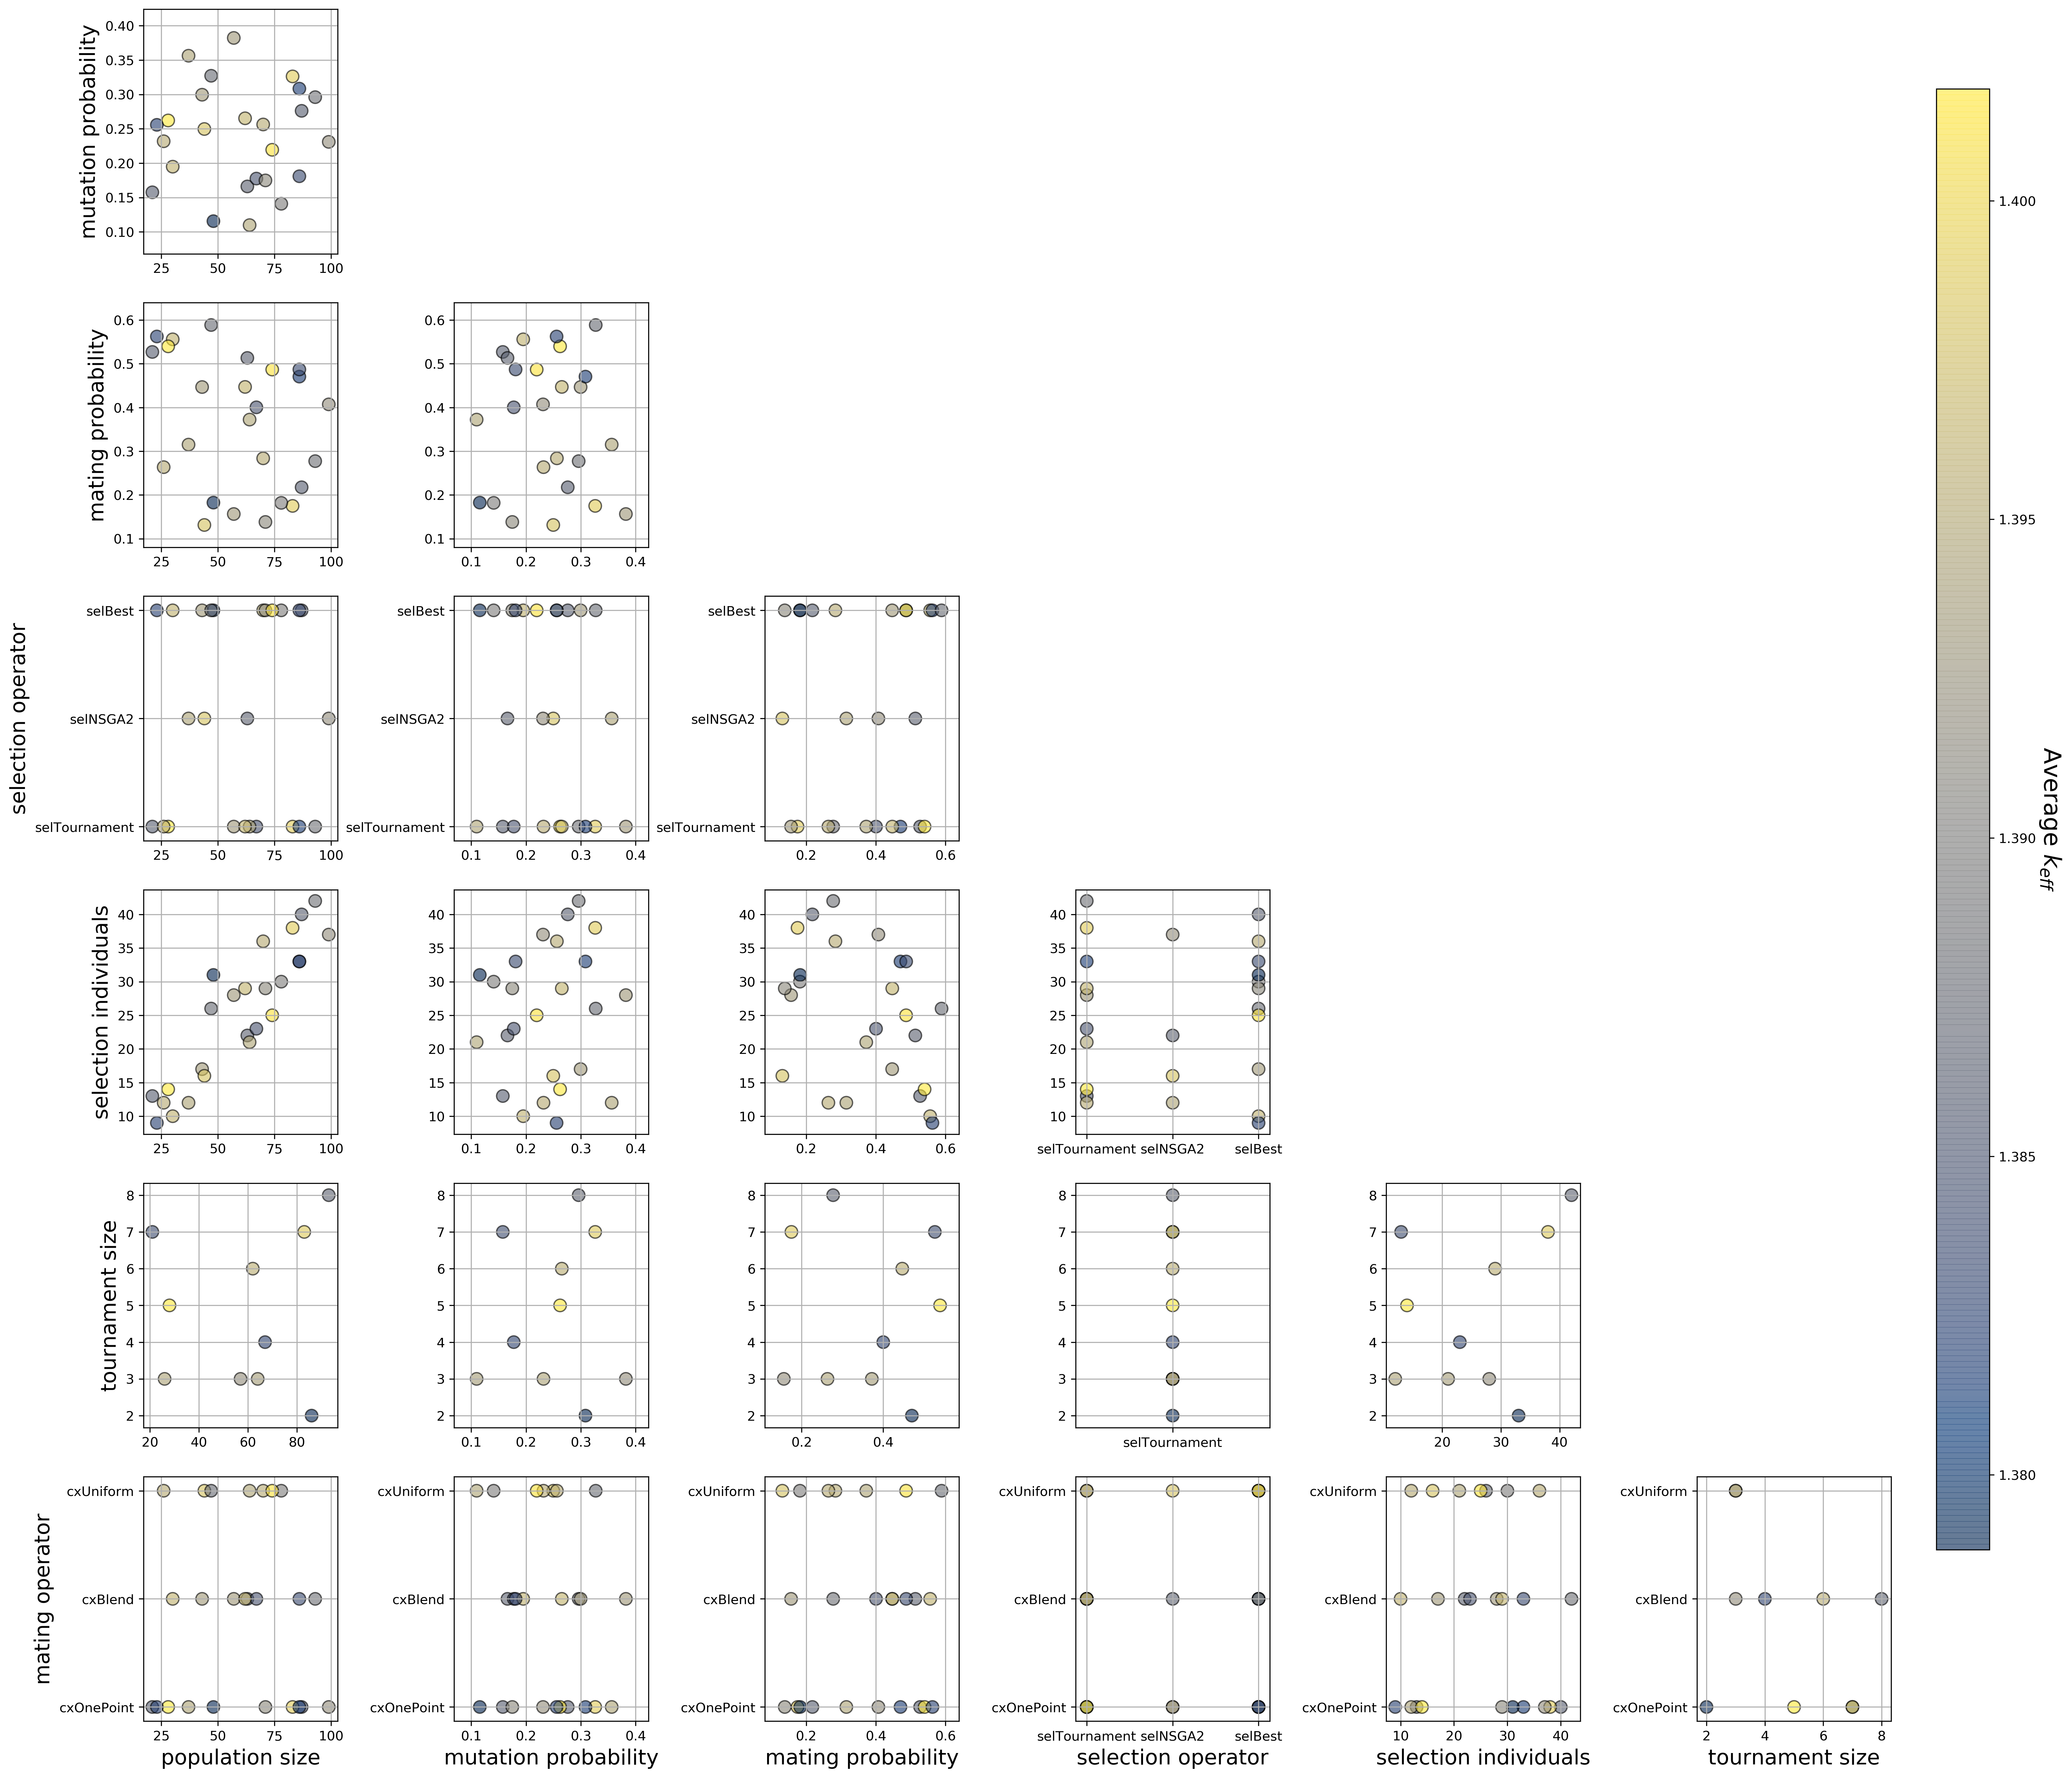
\includegraphics[width=1.3\linewidth]{hyperparameter_sens.png}} 
    \caption{Coarse hyperparameters search's results. Hyperparameter values are plotted 
    against each other with a third dimension of each experiment's final population's 
    average $k_{eff}$ indicated by each scatter point's color.}
    \label{fig:hyperparameter_sens}
\end{figure}
The hyperparameters are plotted against each other to visualize interdependence 
between hyperparameters. 
From the coarse hyperparameter search, the trends that stood out to me were: 
\begin{itemize}
    \item Mutation probability has larger $k_{eff ave}$ between 0.2 and 0.4. 
    \item Mating probability has larger $k_{eff ave}$ when between 0.1 and 0.3. 
    \item Population size has larger $k_{eff ave}$ when between 20 and 60. 
\end{itemize}
There is also not much interdependence between hyperparameters. 

Next, I proceeded to the fine search. 
From Figure \ref{fig:hyperparameter_sens}, I narrowed down population size, 
mutation probability, and mating probability bounds, as shown in Table 
\ref{tab:hyperparameter_search}'s \textit{Fine Search 1 Bounds} column. 
I did not see any significant trends in the other hyperparameters so I chose 
to leave them as is. 
I ran 10 more experiments (25 to 34) with sampling hyperparameters from 
the \textit{Fine Search 1 Bounds}. 
From these results, I conducted a second fine search with 5 experiments 
(35 to 39) with further tuned hyperparameter bounds as shown in Table 
\ref{tab:hyperparameter_search}'s \textit{Fine Search 2 Bounds} column. 
Figure \ref{fig:input_hyperparameters_sens} shows the relationship between 
hyperparameter values and a,b,c input parameters, $k_{eff max}$, and 
$k_{eff ave}$ for each experiment's final generation. 
The coarse experiments' scatter points are $50\%$ transparent, while the fine 
experiments' scatter point are opaque. 
\begin{figure}[]
    \centering
    \makebox[\textwidth][c]{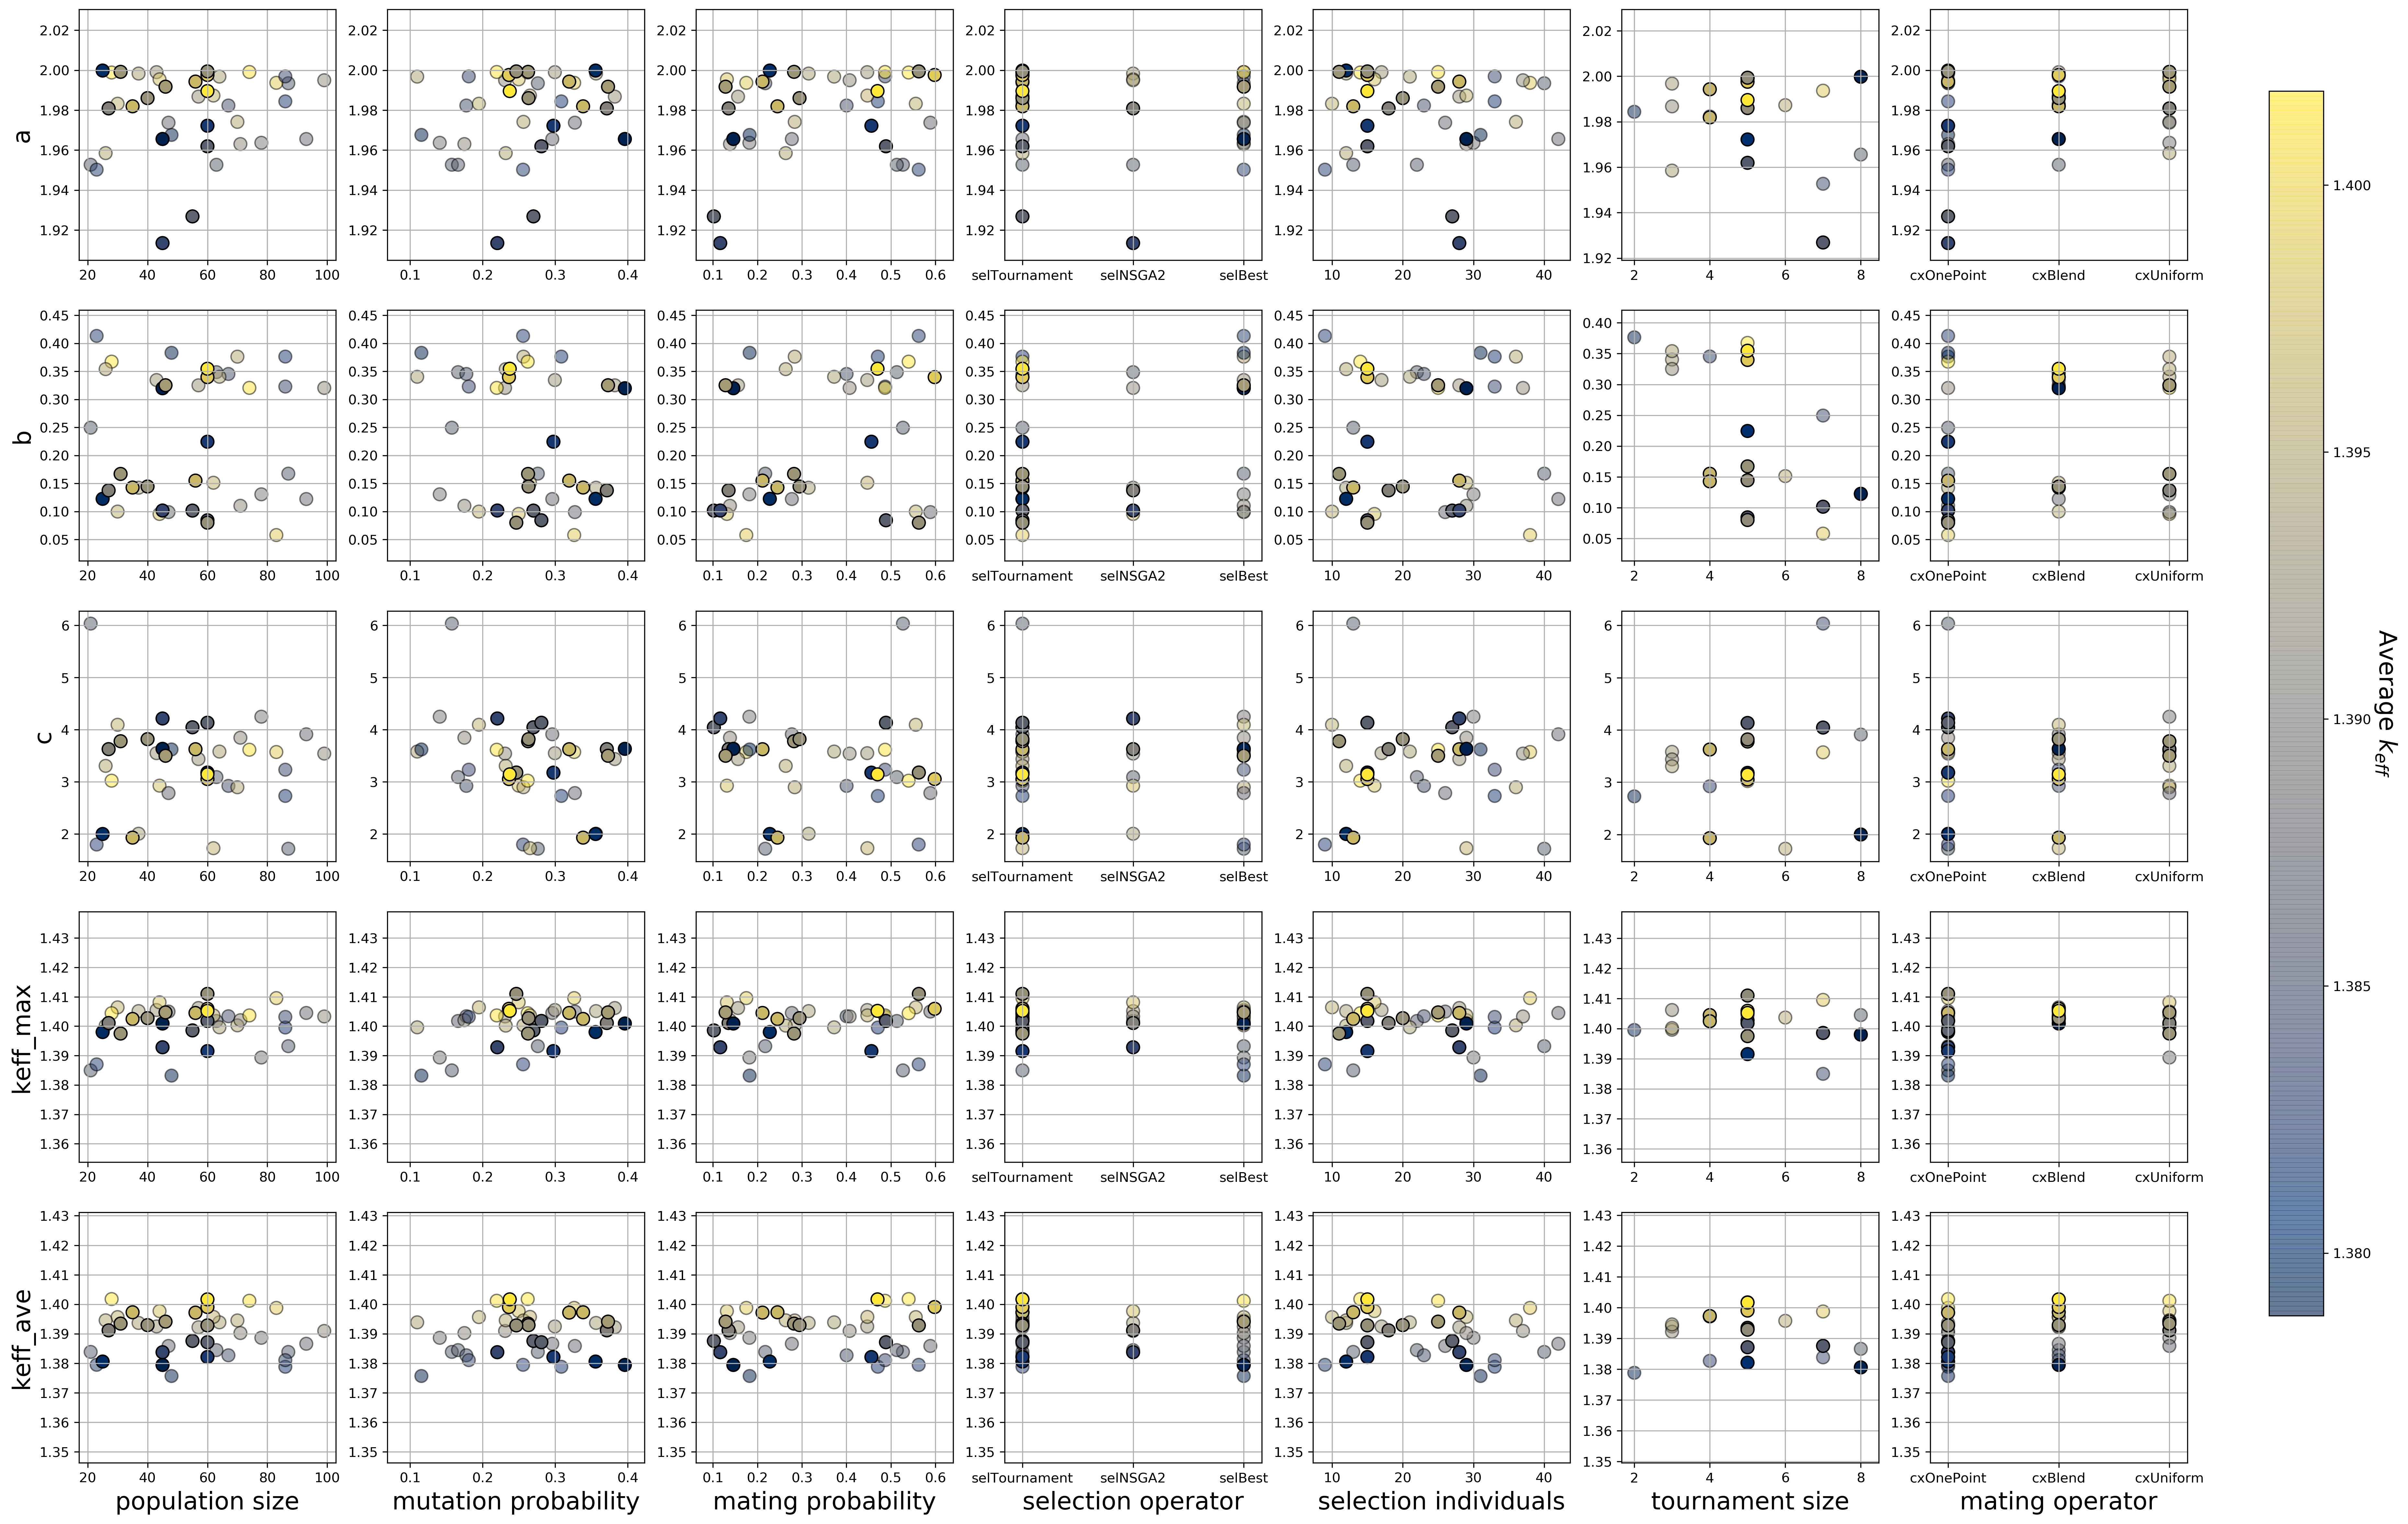
\includegraphics[width=1.3\linewidth]{input_hyperparameters_sens.png}} 
    \caption{Fine hyperparameters search's results. Hyperparameters are plotted 
    against a,b,c input parameters, each experiment's final generation's 
    $k_{eff max}$, and $k_{eff ave}$ with a third dimension of each experiment's 
    final population's average $k_{eff}$ indicated by each scatter point's color.}
    \label{fig:input_hyperparameters_sens}
\end{figure}

Table \ref{tab:topfive} shows the hyperparameters for the five experiments 
with the highest $k_{eff ave}$ for each experiment's final generation.
\begin{table}[]
    \centering
    \onehalfspacing
    \caption{Input and Output Parameters}
	\label{tab:topfive}
    \footnotesize
    \makebox[\textwidth][c]{\begin{tabular}{p{3cm}p{3cm}p{3cm}p{3cm}p{3cm}p{3cm}}
    \hline 
    \textbf{Input/Output Parameters}& \textbf{Experiment 6} & \textbf{Experiment 15} & \textbf{Experiment 24} & \textbf{Experiment 36} & \textbf{Experiment 39}\\
    \hline 
    $k_{eff ave}$ & 1.39876 &1.40175&1.40118&1.39906&1.40165\\ 
    $k_{eff max}$ & 1.40954 &1.40440&1.40365&1.40590&1.40519\\ 
    a & 1.993&1.998&1.999&1.997&1.989\\
    b & 0.057&0.367&0.320&0.339&0.354\\ 
    c & 3.571&3.022&3.615&3.053&3.143\\
    \hline
    \textbf{Hyperparameter}& &&&&\\
    Population size & 83 & 28&74&60&60\\ 
    Generations &8&22&9&10&10 \\
    Mutation probability & 0.32 &0.26&0.21&0.23&0.23\\
    Mating probability & 0.17 &0.53&0.48&0.59&0.46\\
    Selection operator & \texttt{selTournament} &\texttt{selTournament}&\texttt{selBest}&\texttt{selTournament}&\texttt{selTournament}\\
    Selection individuals & 38 &14&25&15&15\\
    Selection tournament size & 7 &5&-&5&5\\
    Mutation Operator & \texttt{mutPolynomial} \texttt{Bounded}&\texttt{mutPolynomial} \texttt{Bounded}&\texttt{mutPolynomial} \texttt{Bounded}&\texttt{mutPolynomial} \texttt{Bounded}&\texttt{mutPolynomial} \texttt{Bounded}\\
    Mating Operator & \texttt{cxOnePoint} &\texttt{cxOnePoint}&\texttt{cxUniform}&\texttt{cxBlend}&\texttt{cxBlend}\\ 
    \hline
    \end{tabular}}
\end{table}
Figure \ref{fig:topfiveplot} shows the packing fraction distributions that 
produced the $k_{eff max}$ from each of the top five experiments. 
\begin{figure}[]
    \centering
    \makebox[\textwidth][c]{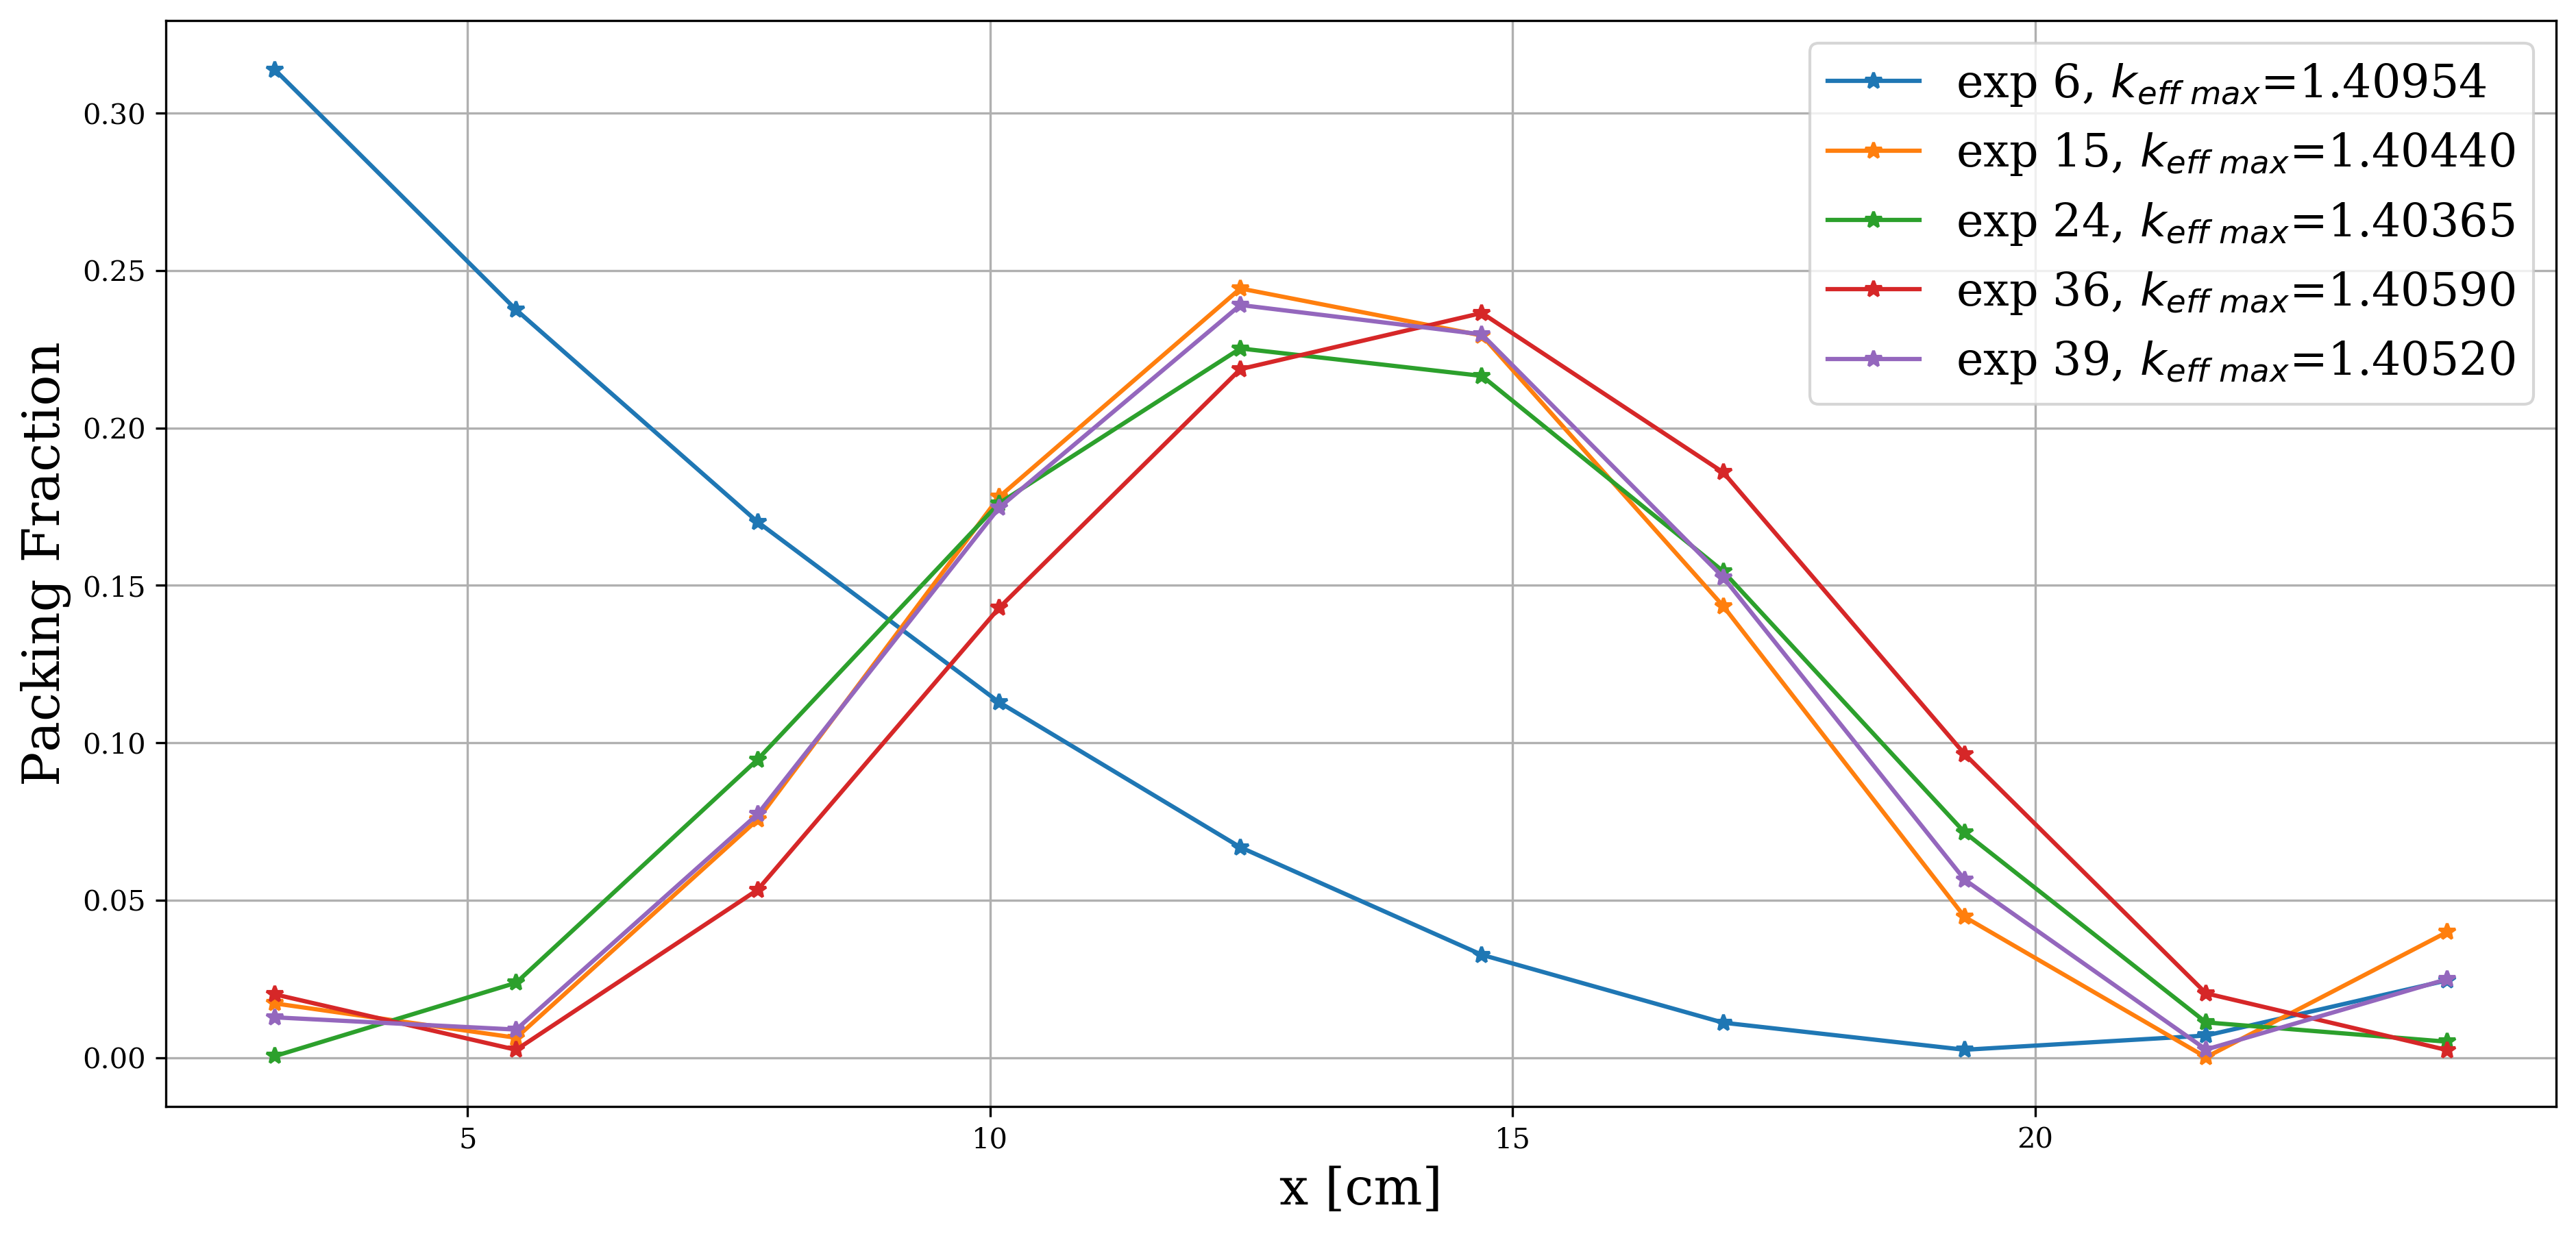
\includegraphics[width=1\linewidth]{topfive_plot.png}} 
    \caption{}
    \label{fig:topfiveplot}
\end{figure}
Four experiments had similar distributions of packing fraction peaking at approximately 
0.23 in the centre of the slab, while one experiment had an exponential-looking 
distribution with peak packing fraction of 0.31 at side of the slab.
This demonstrates the robustness of the genetic algorithms to find similar solutions with 
different hyperparameters. 

\subsection{Results for best hyperparameter set}
The best performing set of hyperparameters are from the final 
\textit{Fine Search 2} and is experiment 39 in Table \ref{tab:topfive}
with centre-peaking packing fraction distribution with $k_{eff max} = 1.40519$. 
Experiment 39's $k_{eff max}$ is $\sim2000$pcm larger than the original 
straighted \gls{AHTR} configuration's $k_{eff}$. 

Figure \ref{fig:keff_conv_39} and \ref{fig:pf_39} show the evolution of $k_{eff}$ 
and packing fraction distribution through each generation of the best performing 
39$^{th}$ experiment, respectively. 
\begin{figure}[]
    \centering
    \begin{subfigure}{\textwidth}
    \makebox[\textwidth][c]{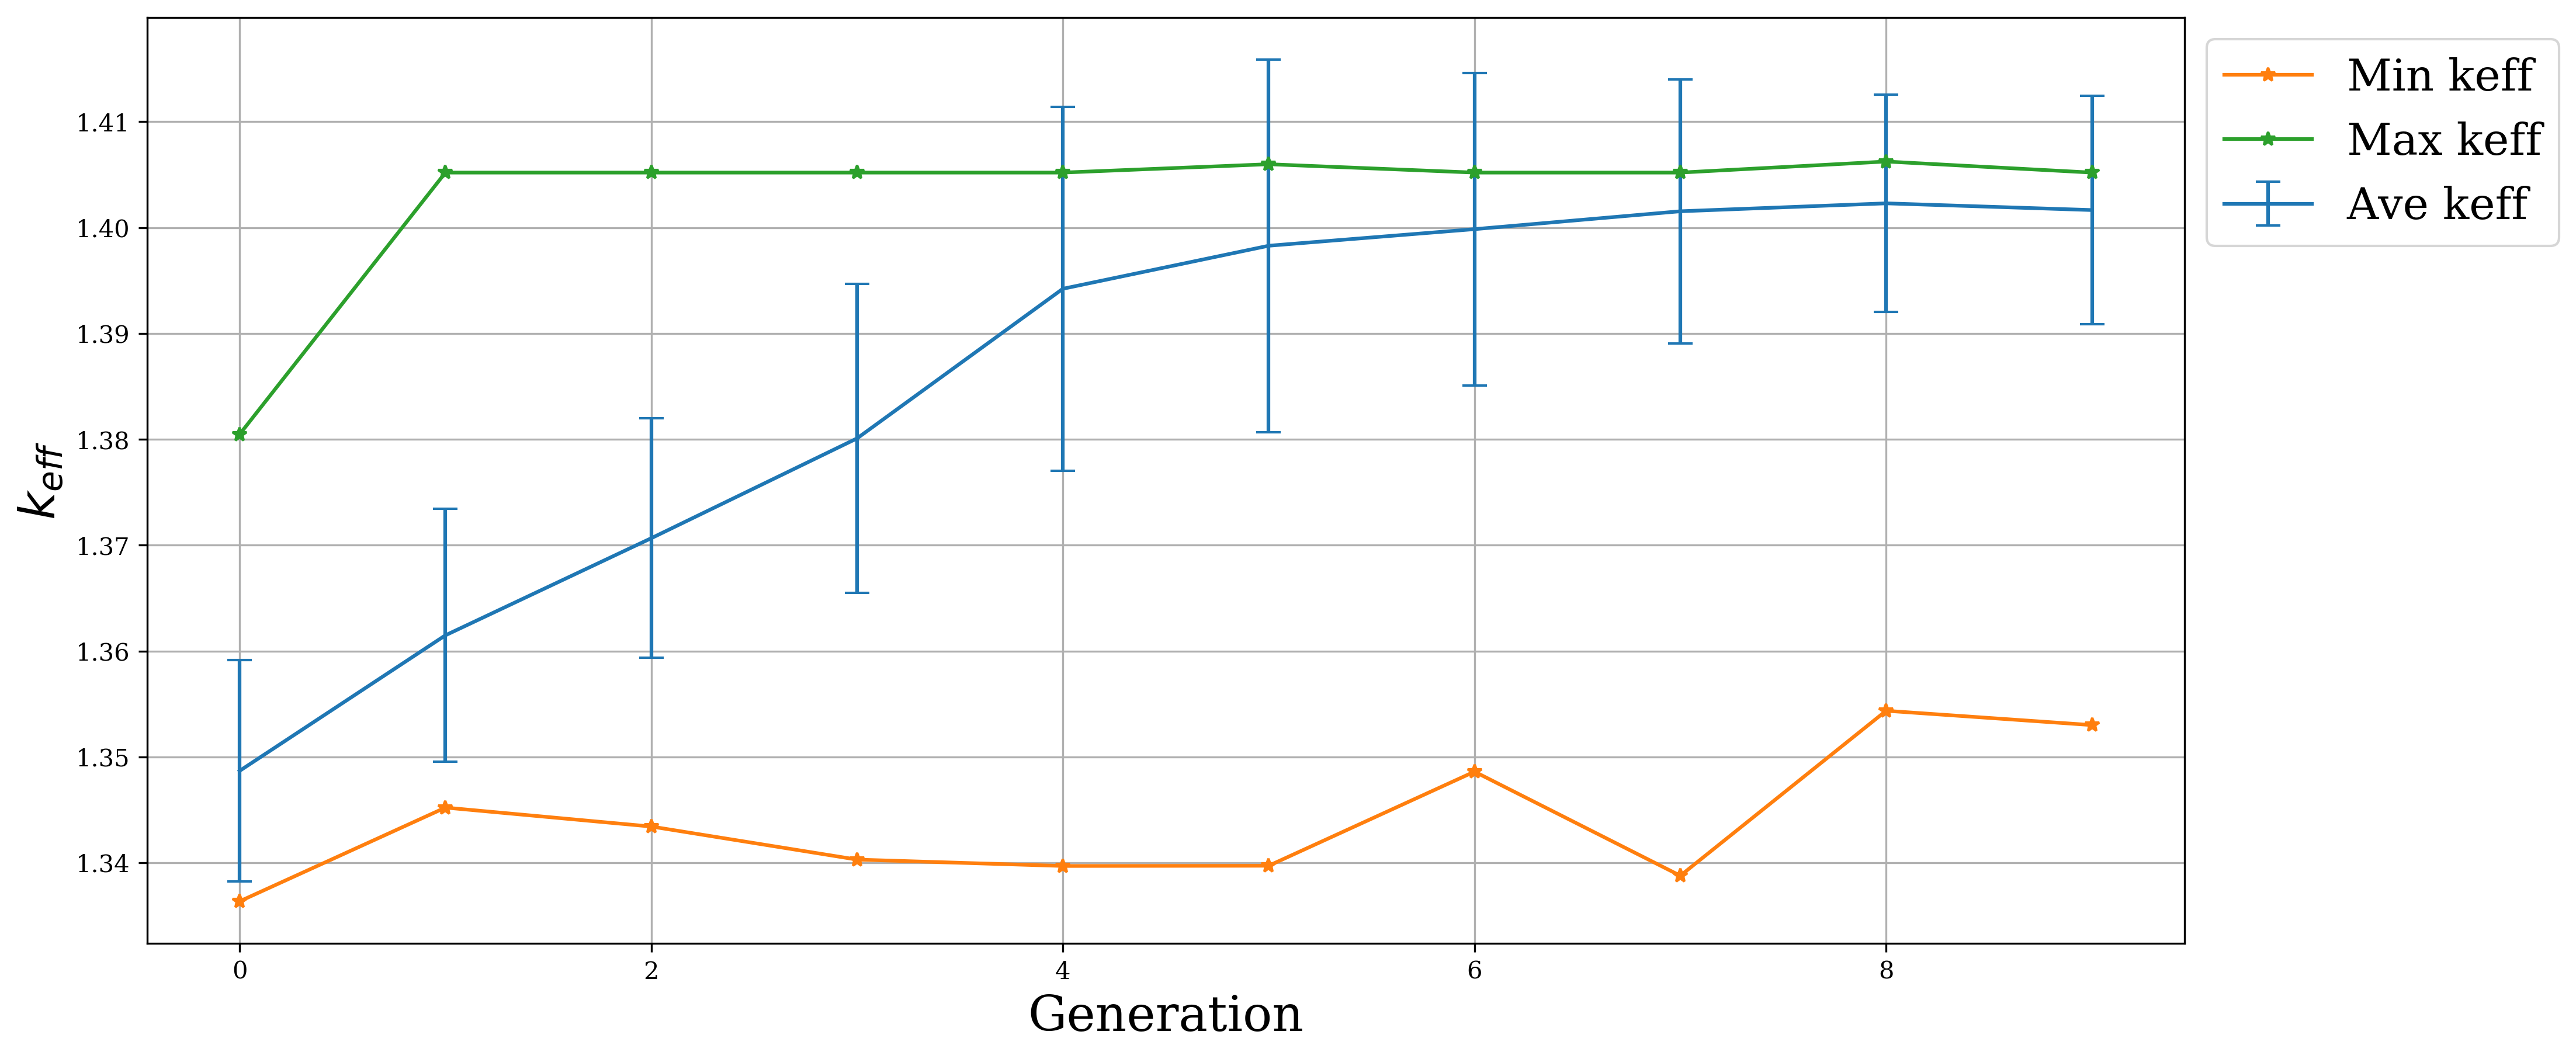
\includegraphics[width=1.1\linewidth]{keff_conv_39.png}} 
    \caption{Minimum, average, and maximum $k_{eff}$ values evolution.}
    \label{fig:keff_conv_39}
    \end{subfigure}
    \begin{subfigure}{\textwidth}
        \makebox[\textwidth][c]{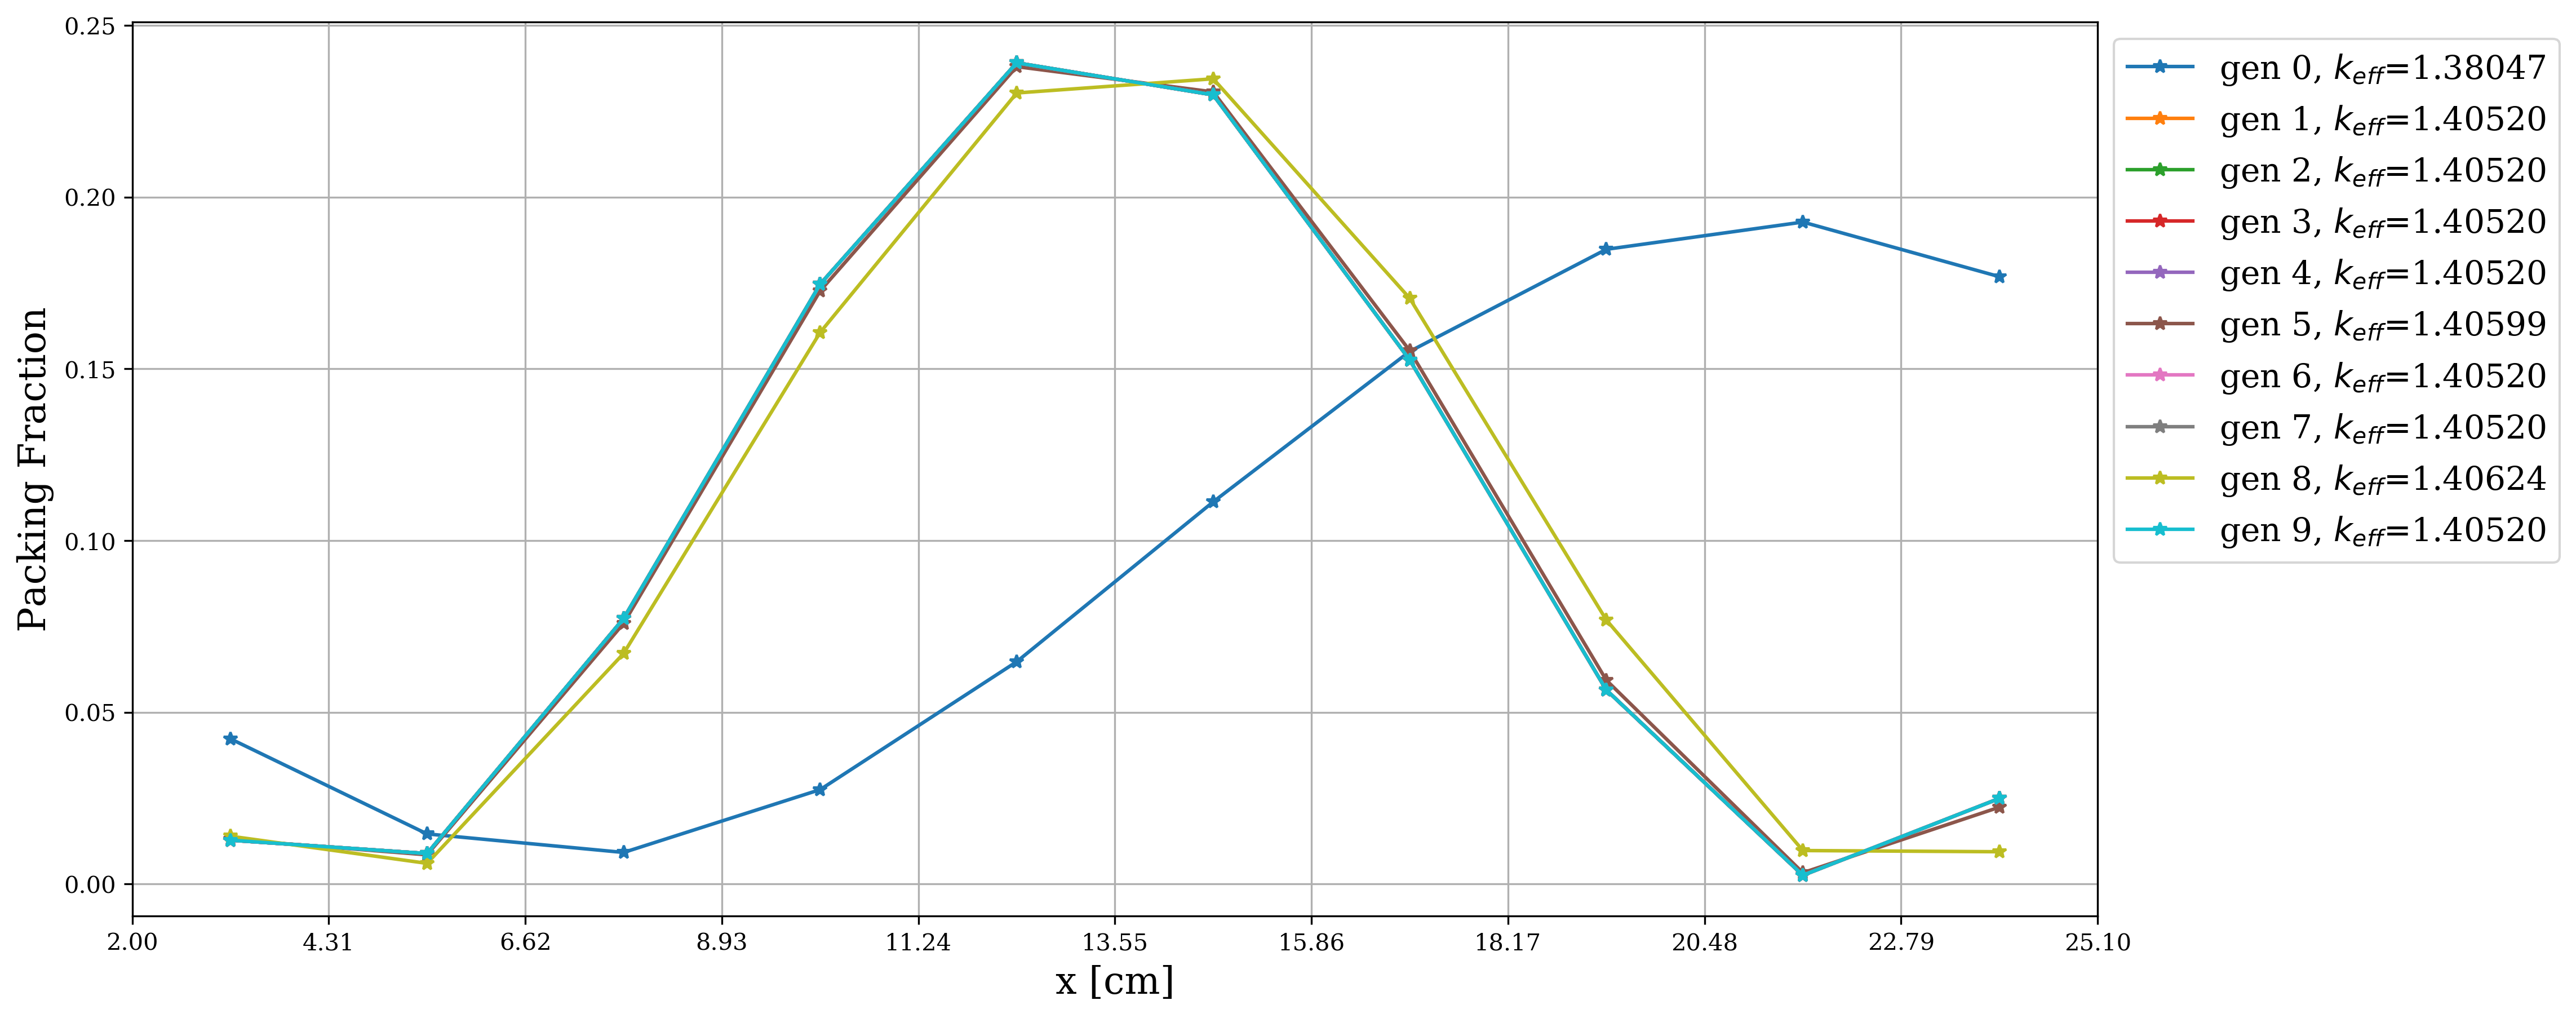
\includegraphics[width=1.1\linewidth]{pf_39.png}} 
        \caption{Maximum $k_{eff}$'s packing fraction distribution evolution.}
        \label{fig:pf_39}
    \end{subfigure}
    \caption{ Results for each generation for REALM's genetic algorithm optimization 
    of the Straightened \acrfull{AHTR} Fuel Slab. The REALM simulation used 
    the 39$^{th}$ experiment's hyperparameter set.}
    \label{fig:39}
\end{figure}
The maximum $k_{eff}$ converged quickly by generation 1, however, this is not 
usually the case. 
The genetic algorithm optimization process is stochastic, and so there is always 
the possibility that the algorithm randomly samples a set of input parameters
that maximizes the objective function. 
The average $k_{eff}$ shows how the average population of individuals converge 
towards a higher $k_{eff}$ with improvements from each generation. 
Figure \ref{fig:keff_conv_15} and \ref{fig:pf_15} show the evolution of $k_{eff}$ 
and packing fraction distribution through each generation of the second best 
performing 15$^{th}$ experiment, respectively. 
Experiment 15 demonstrates how both maximum and average $k_{eff}$ converges 
towards a higher $k_{eff}$ with improvements from each generation.
\begin{figure}[]
    \centering
    \begin{subfigure}{\textwidth}
    \makebox[\textwidth][c]{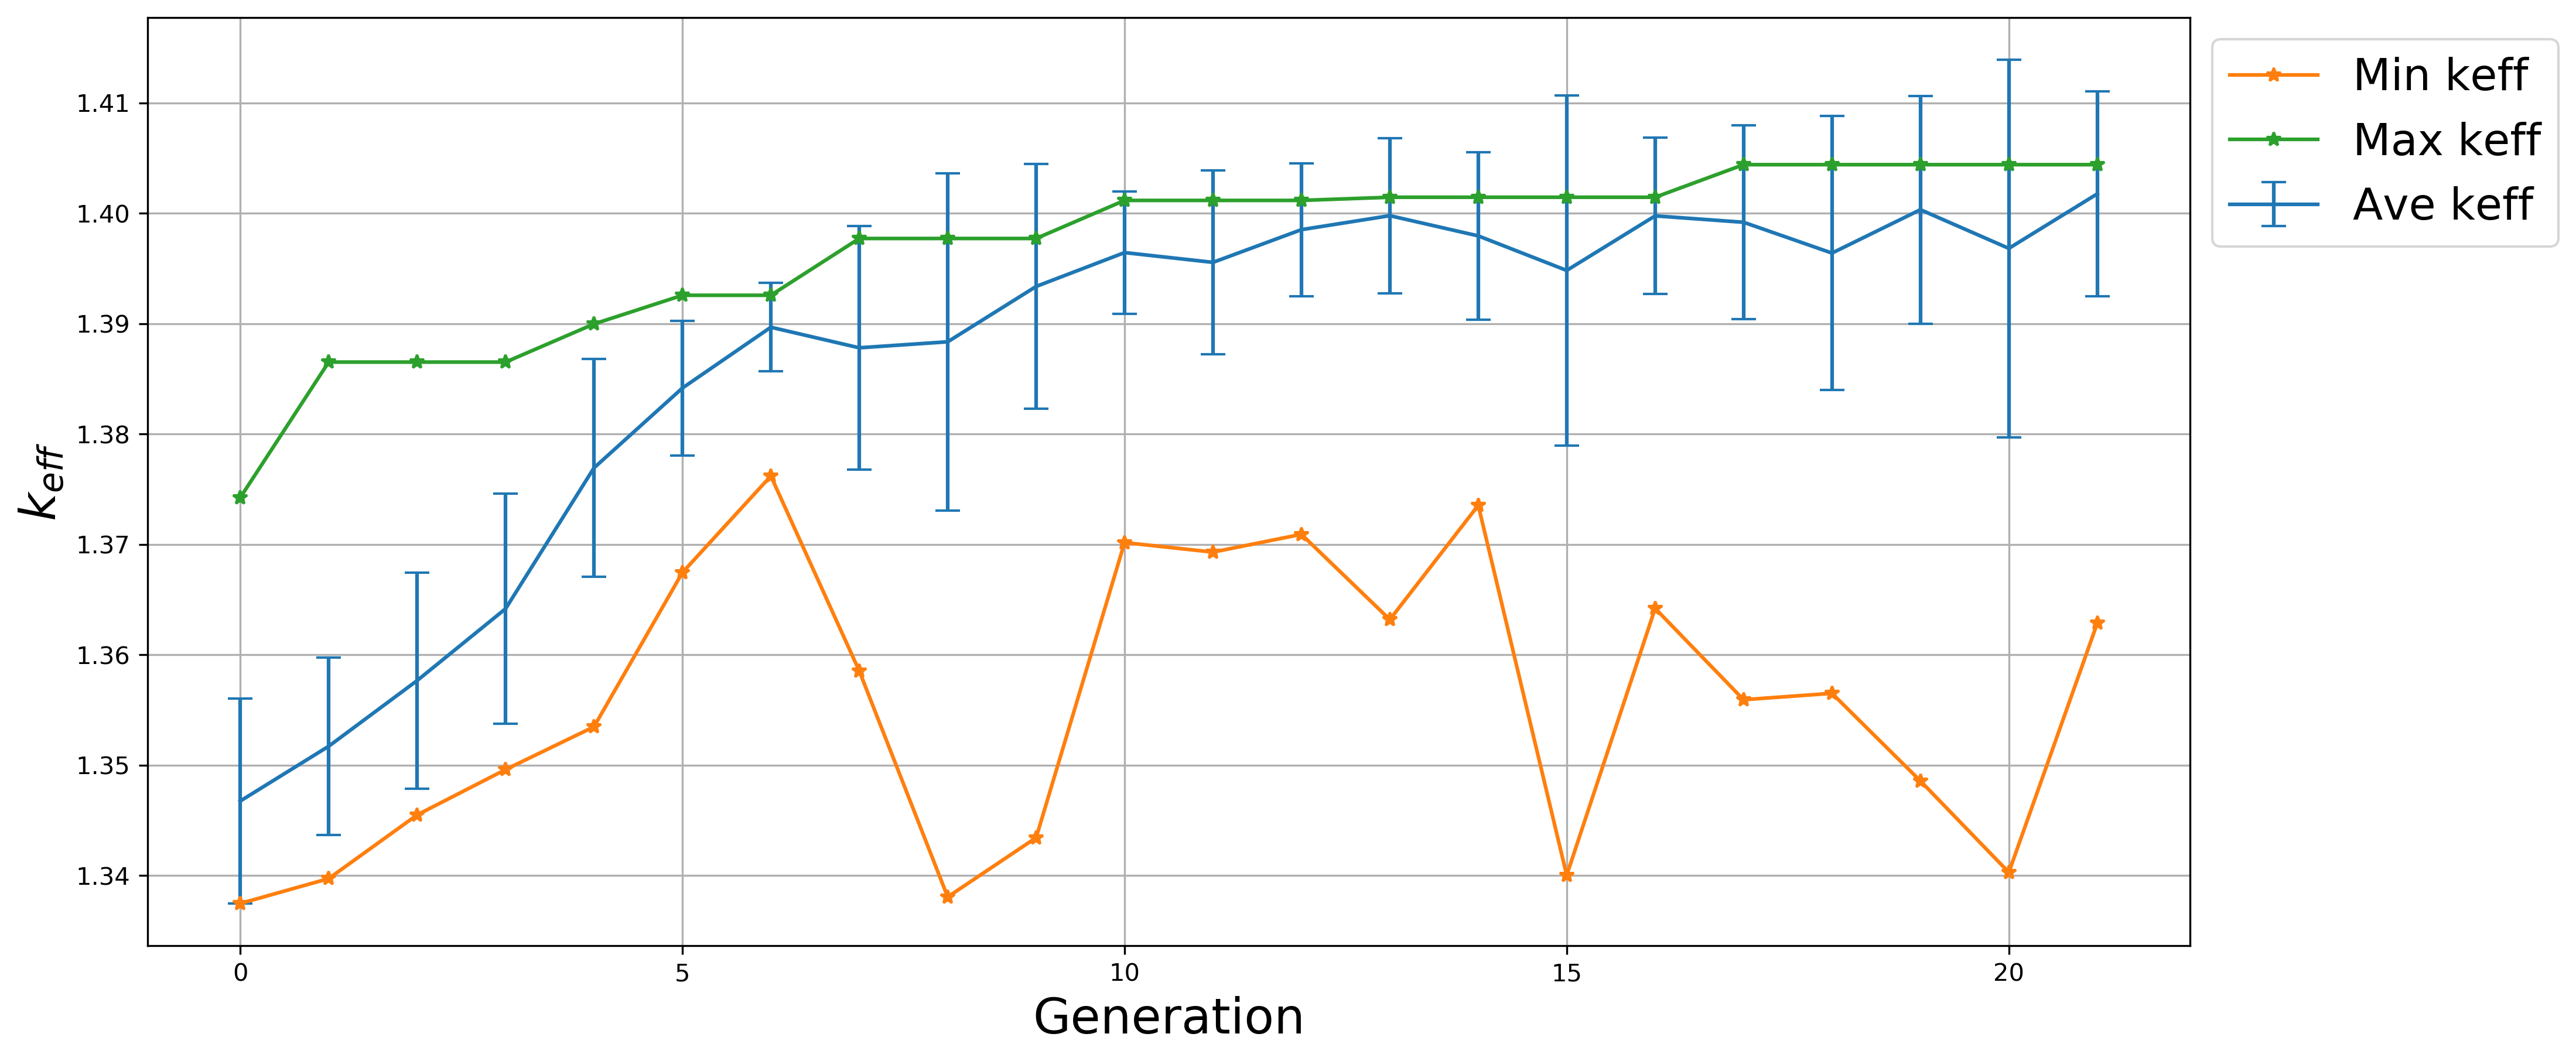
\includegraphics[width=1.1\linewidth]{keff_conv_15.png}} 
    \caption{Minimum, average, and maximum $k_{eff}$ values evolution.}
    \label{fig:keff_conv_15}
    \end{subfigure}
    \begin{subfigure}{\textwidth}
        \makebox[\textwidth][c]{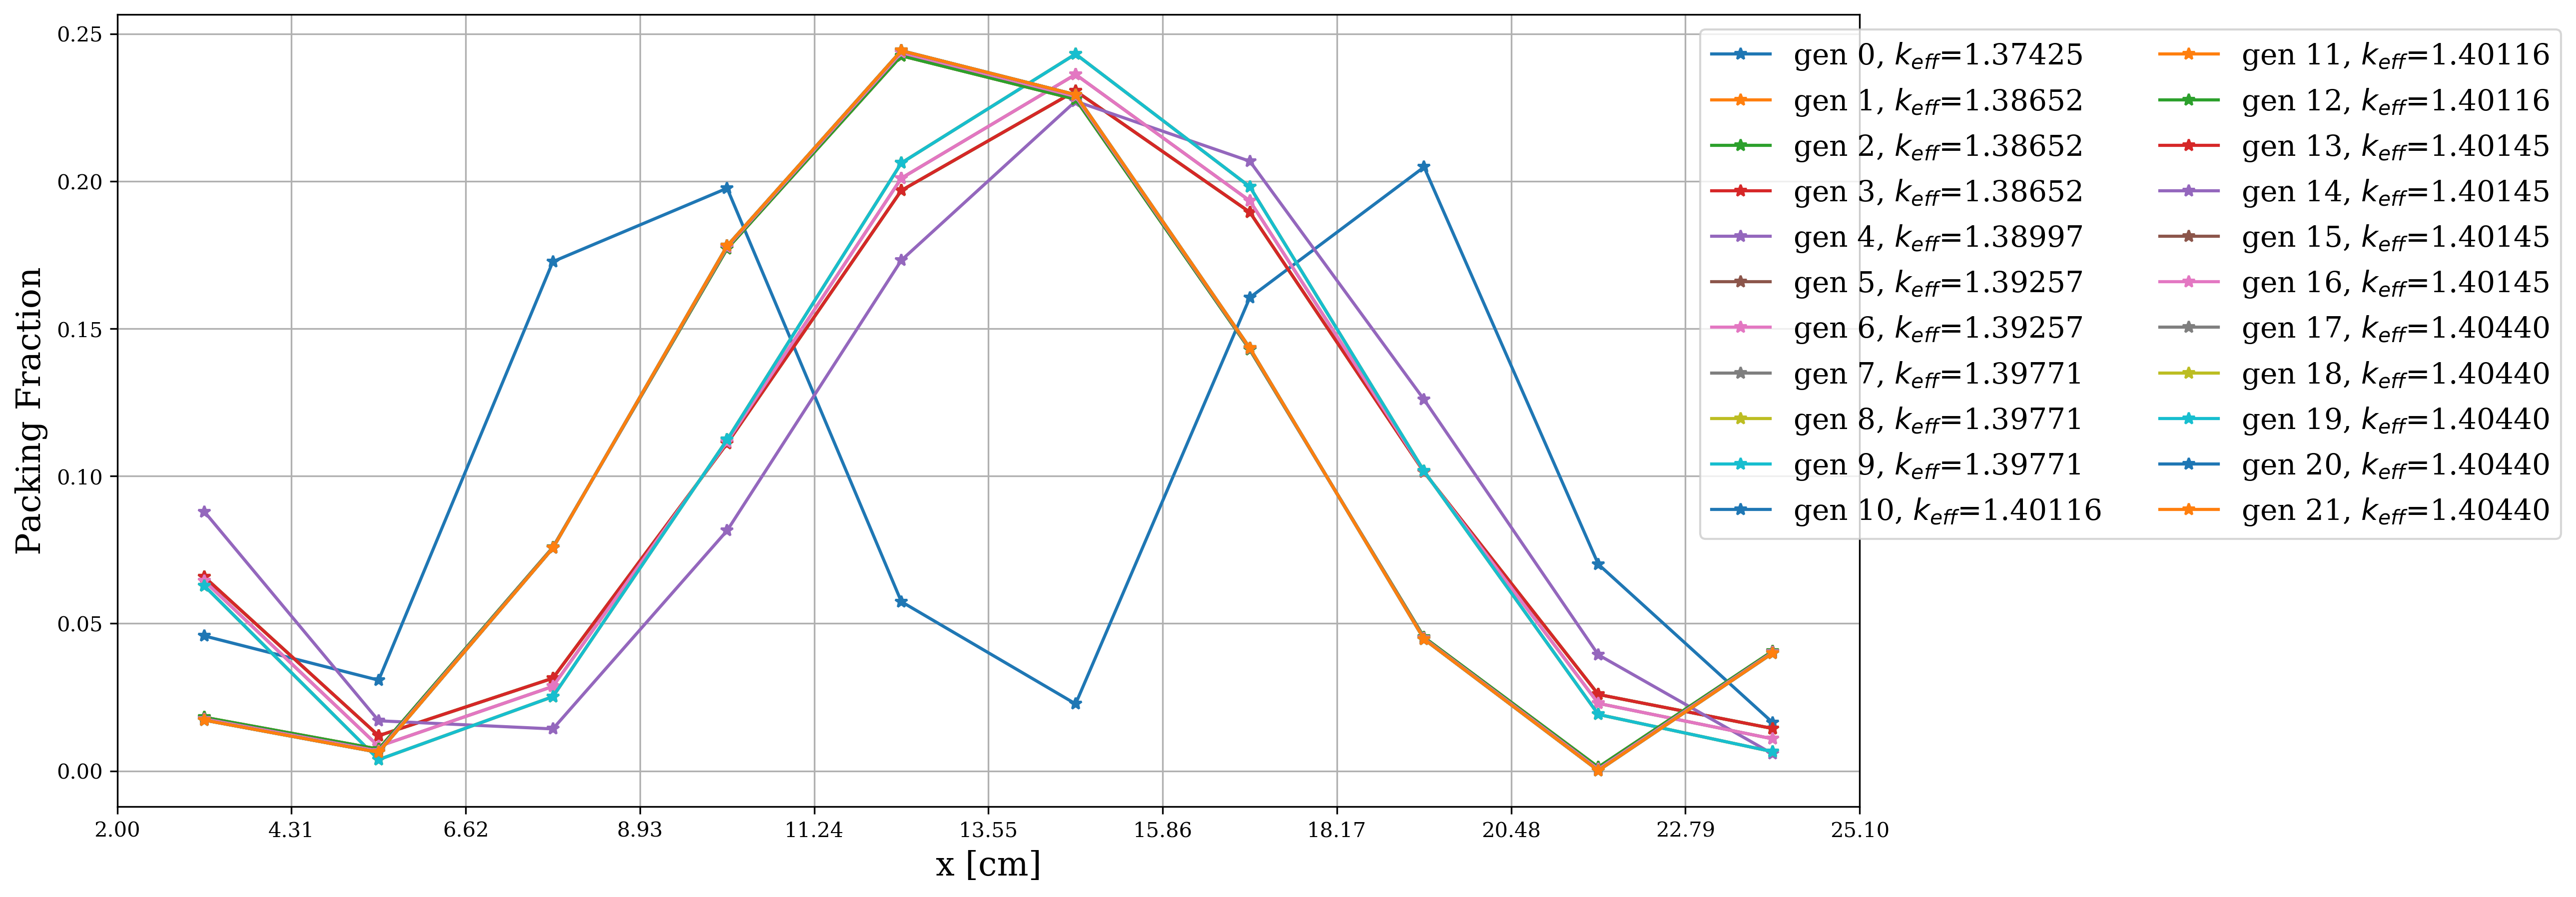
\includegraphics[width=1.1\linewidth]{pf_15.png}} 
        \caption{Maximum $k_{eff}$'s packing fraction distribution evolution.}
        \label{fig:pf_15}
    \end{subfigure}
    \caption{ Results for each generation for REALM's genetic algorithm optimization 
    of the Straightened \acrfull{AHTR} Fuel Slab. The REALM simulation used 
    the 15$^{th}$ experiment's hyperparameter set.}
    \label{fig:15}
\end{figure}
% convergence of keff
% explain why this distribution makes sense. 